\documentclass[professionalfont]{beamer}
\usetheme{Berlin}
% \usecolortheme{dove}
\beamertemplatenavigationsymbolsempty
\setbeamertemplate{footline}[frame number]
\setbeamertemplate{caption}[numbered]

\setbeamercovered{highly dynamic}

\newcounter{saveenumi}
\newcommand{\seti}{\setcounter{saveenumi}{\value{enumi}}}
\newcommand{\conti}{\setcounter{enumi}{\value{saveenumi}}}

\usepackage{bbm}
\usepackage{amsmath}
\usepackage{xcolor}
\usepackage{listings}
\usepackage{natbib}
\usepackage{epsfig,latexsym,amssymb}
\usepackage{newtxtext,newtxmath}
\usepackage{multirow}

\usepackage{amscd}
\usepackage{graphicx}
\usepackage{lscape}
\usepackage{picture, eso-pic, tikz} %% for gray boxes
\usepackage{dsfont}
\usepackage{natbib}
\usepackage{arydshln}


\def\RR{{\mathbb R}}  %%
\def\R{{\mathbb R}}  %%
\def\N{{\mathbb N}}  %%
\def\p{{\mathbb P}}  %%
\def\Z{{\mathbb Z}}  %%
\def\Q{{\mathbb Q}}  %%
\def\C{{\mathbb C}}  %%
\def\E{{\mathbb E}}  %
\def\F{{\mathbb F}}  %%
\def\Va{{\mathbb V}}  %%

\lstset{language=R,basicstyle=\ttfamily\tiny,breaklines=true}

%\newcommand{\R}[1]{\small {\colorbox{lightgray}{\texttt{#1}}}}
%\newcommand{\Rout}[1]{\textcolor{green}{\small \textrm{#1}}}

\def\bx{\boldsymbol{x}}
\def\bX{\boldsymbol{X}}

\def\bz{\boldsymbol{z}}
\def\bw{\boldsymbol{w}}
\def\bZ{\boldsymbol{Z}}
\def\bY{\boldsymbol{Y}}
\newcommand{\blue}[1]{\textcolor{blue}{#1}}
\newcommand{\gray}[1]{\textcolor{gray}{#1}}
\newcommand{\red}[1]{\textcolor{red}{#1}}
\newcommand{\green}[1]{\textcolor{green}{#1}}
\usepackage{newtxtext,newtxmath}

\title{Gradient tree-boosted mixture models and their applications in insurance loss prediction}

\author{GAO, Guangyuan\footnote{Joint work with Li, Jiahong (Peking University)}}
%\institute{School of Statistics, Renmin University of China}
%\date{The 120th Lecture of Statistics, June 10, 2020}

%\subtitle{A perspective from actuarial science and risk management}
%\author{GAO, Guangyuan}
\institute{Center for Applied Statistics and School of Statistics, Renmin University of China}
\date{Department of Mathematics at SUSTech, November 2021}



\begin{document}
\begin{frame}
\titlepage
\end{frame}

%\AtBeginSection[]
%{
%    \begin{frame}
%        \tableofcontents[currentsection]
%    \end{frame}
%}

\begin{frame}{Table of Contents}
\tableofcontents
\end{frame}

\section{Motivations}
\begin{frame}{Insurance loss}

Insurance loss data sometimes cannot be well modeled by a single distribution.
\begin{itemize}
	\item For claims counts data, there may be an excess of zero claims, so a Poisson distribution is not the best choice.
	\item For claims amount data, there may be a heavy tail, so a gamma distribution is not enough to describe the entire data.
	\begin{figure}[h!]
		\centering
		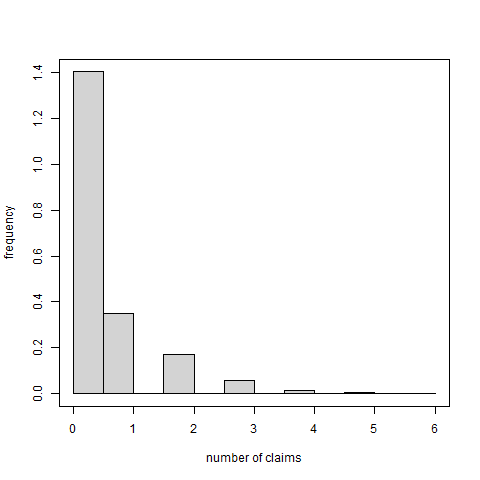
\includegraphics[width=0.3\linewidth]{../plots/zip/hist_poisson.png}
		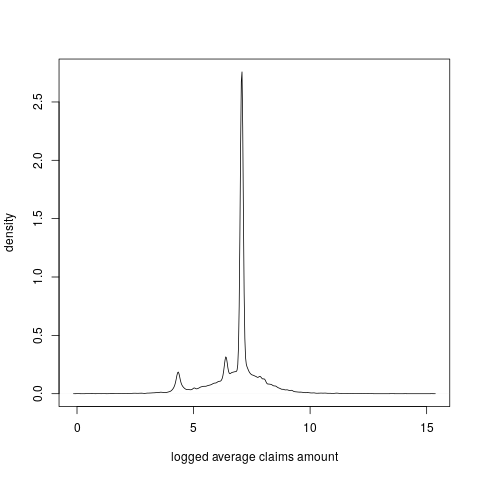
\includegraphics[width=0.3\linewidth]{../plots/sev/hist.png}
	\end{figure}
\end{itemize}

One solution is to apply \blue{mixture of distributions}.
\end{frame}

\begin{frame}{Insurance loss}

	\begin{itemize}
		\item For claims counts data, we can utilize \blue{zero-modified Poisson} distribution.
		\item For claims amount data, we can utilize \blue{mixture of gamma distribution and heavy-tailed distribution} such as Pareto distribution.
	\end{itemize}
	When the individual risk factors are available, we can extend mixture of distributions to \blue{mixture of regressions} to address  risk heterogeneity in the portfolio.
\end{frame}

\begin{frame}{Challenges with mixture models}



	\begin{itemize}
		\item \blue{Parameter estimation} in mixture models is challenging: each {component distribution/regression} parameters are related to each other.
		%\item The \blue{expectation-maximization algorithm} is an iterative method to estimate component parameters and {(hidden) component indicator variable}.
		\item \blue{Variable selection} in mixture models is also challenging:
		we need to perform variable selection for each component regression.
	\end{itemize}
	\end{frame}



 \section{Reviews: Mixture of models and EM algorithm}
 \subsection{Mixture of models}

 \begin{frame}{Mixture of distributions}
Suppose a random variable $y$ follows the $k$-th \blue{component distribution} from
$$\{f_1(y;\mu_1,\phi_1),\ldots,f_K(y;\mu_K,\phi_K)\}$$
with \blue{mixing probability} $p_k, k=1,\ldots,K$,
then the probability density function for $y$ is
$$f(y)=\sum_{k=1}^Kp_kf_k(y;\mu_k,\phi_k).$$
\end{frame}

 \begin{frame}{Mixture of regressions}
 	If \blue{individual features $\bx_i$} are available and they have systematic effects on the distribution of $y_i$, then we establish a mixture of regressions:
 	$$f(y|\bx)=\sum_{k=1}^Kp_k(\bx)f_k(y;\mu_k(\bx),\phi_k(\bx)).$$

 	Above is the most general form of mixing. 	In applications, we always put some constraints on the \blue{mixing structure}.
 \end{frame}

  \begin{frame}{Mixing structures}

 	\begin{itemize}
 		\item Mixing probabilities are not related to $\bx$
 		$$f(y)=\sum_{k=1}^Kp_kf_k(y;\mu_k(\bx),\phi_k(\bx)).$$
 		\item Both mixing probabilities and dispersions are not related to $\bx$
 		 	$$f(y)=\sum_{k=1}^Kp_kf_k(y;\mu_k(\bx),\phi_k),$$
 		 	 	\end{itemize}
 	 	 \end{frame}

  \begin{frame}{Mixing structures}

	\begin{itemize}
 		\item If component distributions are from the same distribution family, we might assume different component distributions have the same dispersion
 		 	$$f(y)=\sum_{k=1}^Kp_kf_k(y;\mu_k(\bx),\phi).$$
 		 \item Covariates $\bx$ are only related to the mixing probabilities:
 		  	$$f(y)=\sum_{k=1}^Kp_k(\bx)f_k(y;\mu_k,\phi_k).$$
 	\end{itemize}

We need to determine the mixture structure according to the data and our aim. Imposing suitable constraints on mixture, we can \blue{accelerate model fitting} without compromising predictive performance.

\end{frame}

\subsection{EM algorithm}

\begin{frame}{Likelihood function given full information}
Suppose we know which component distribution each sample is from. That is we know the \blue{full information} $(Y,Z,\bx)$ where
$$Z=(Z_1,\ldots,Z_K)^\top=(\mathbbm{1}_1(k),\ldots,\mathbbm{1}_K(k))^\top$$
is the one-hot encoding of \blue{component indicator variable}.


The joint distribution function for full information (one sample) is given by
	$$f(y,z|
	\bx) = \prod_{k=1}^K\left[p_k(\bx)f_k(y;\mu_k(\bx),\phi_k(\bx))\right]^{z_k}$$
The \blue{log-likelihood function} is given by
\begin{equation}\label{full-L}
		l(p,\mu,\phi|y,z,\bx)=\sum_{k=1}^K z_k\left[\log p_k(\bx) + \log f_k(y;\mu_k(\bx),\phi_k(\bx))\right]
\end{equation}
\end{frame}

\begin{frame}{Likelihood function given full information}
	The parameters in $p,\mu,\phi$ can be estimated by $K+1$ \blue{independent optimizations}
	\begin{equation}\label{p-reg}
		\hat{\theta}_p=\underset{\theta_p}{\arg\max}\sum_{i=1}^n\sum_{k=1}^Kz_{i,k}\log p_k(\bx_i;\theta_p)
	\end{equation}
	\begin{equation}\label{comp-reg}
		\left(\hat{\theta}_\mu^{(k)},\hat{\theta}_\phi^{(k)}\right)=\underset{\theta^{(k)}_\mu,\theta^{(k)}_\phi}{\arg\max}\sum_{i=1}^n\sum_{k=1}^Kz_{i,k}\log f_k\left(y_i;\mu_k\left(\bx_i;\theta_\mu^{(k)}\right),\phi_k\left(\bx_i;\theta_\phi^{(k)}\right)\right)
	\end{equation}
\end{frame}

\begin{frame}{Likelihood function given full information}
Those optimizations are corresponding to  \blue{a multinomial logistic classification} and \blue{$K$ regressions}.

~

The multinomial logistic classification are fitted to all samples, while $K$ regressions are fitted to {partial} samples with $\{i:z_{i,k}=1\}$.
\end{frame}

\begin{frame}{Expectation step}


	With iterated $\hat{p},\hat{\mu},\hat{\phi}$, calculate the \blue{conditional expectation} of $z$:
		$$\hat{z}_{i,k}=\hat{z}_k(\bx_i)=\frac{\hat{p}_{i,k}f_k(y_i;\hat{\mu}_{i,k},\hat{\phi}_{i,k})}{\sum_{l=1}^K\hat{p}_{i,l}f_l(y_i;\hat{\mu}_{i,l},\hat{\phi}_{i,l})},$$
		where
		$\hat{p}_{i,k}=\hat{p}_k(\bx_i),\hat{\mu}_{i,k}=\hat{\mu}_k(\bx_i),\hat{\phi}_{i,k}=\hat{\phi}_k(\bx_i)$.
\end{frame}

\begin{frame}{Maximization step}
Based on the following likelihood function for full information, calculate the MLE of parameters.
	\begin{equation}
		\begin{aligned}
			&l(p,\mu,\phi|y,\hat{z},\bx)\\
			=&\sum_{i=1}^n\sum_{k=1}^K \hat{z}_{i,k}\left[\log p_k(\bx_i) + \log f_k(y_i;\mu_k(\bx_i),\phi_k(\bx_i))\right]\\
			=&\sum_{i=1}^n\sum_{k=1}^K \hat{z}_{i,k}\log p_k(\bx_i) + \sum_{i=1}^n\sum_{k=1}^K \hat{z}_{i,k}\log f_k(y_i;\mu_k(\bx_i),\phi_k(\bx_i))
		\end{aligned}
	\end{equation}
This step is similar to \eqref{p-reg} and \eqref{comp-reg}. However, now we have $\hat{z}_{i,k}\in(0,1)$, so we need to consider
\begin{itemize}
	\item A multinomial logistic classification with \blue{fractional} response.
	\item $K$ \blue{weighted}-regressions fitted to \blue{all} samples.
\end{itemize}
\end{frame}

\section{Expectation-Boosting algorithm}



\subsection{Generic functional gradient descent algorithm}
\begin{frame}{Our proposal}
	
	We replace the maximization step in the EM algorithm by a \blue{boosting step}.
	
	~
	
	The boosting step  increases the likelihood, but \blue{overfitting-sensitively}.
	
	
	~
	
	The boosting step follows a \blue{generic functional gradient descent algorithm}.
	
\end{frame}
\begin{frame}{General setting}
	Suppose \blue{non-parametric regression function} as $F:\R^P\rightarrow\R$. Our purpose is to  estimate $F$ to minimize the expected loss $$\hat{F}=\underset{F}{\arg\min}\E\left[C(Y,F(\bx))\right],$$
	where $C:\R\times\R\rightarrow\R_+$ is the \blue{loss function}.

	~

	We always replace the expected loss by sample average loss:
	$$\hat{F}=\underset{F}{\arg\min} \frac{1}{n}\sum_{i=1}^nC(y_i,F(\bx_i))$$
\end{frame}

\begin{frame}{Link functions and loss functions}

	Commonly used \blue{link function} and loss functions:
	\begin{itemize}
		\item AdaBoost: $$C(y,F)=\exp(yF),  ~~ y\in\{-1,1\}$$
		$$F(\bx)=\frac{1}{2}\log\left(\frac{\Pr[Y=1|\bx]}{\Pr[Y=-1|\bx]}\right)$$
		\item LogitBoost: $$C(y,F)=\log_2(1+\exp(-2yF)), ~~ y\in\{-1,1\}$$
		$$F(\bx)=\frac{1}{2}\log\left(\frac{\Pr[Y=1|\bx]}{\Pr[Y=-1|\bx]}\right)$$
		\item $L_2$Boost: $$C(y,F)=(y-F)^2/2, ~~ y\in \R$$
		$$F(\bx)=\E(Y|\bx)$$
	\end{itemize}
\end{frame}

\begin{frame}{Loss function for insurance data}
	We choose the \blue{negative log-likelihood} function as the loss function. Hence, minimizing the loss function is equivalent to maximizing the likelihood function.
\end{frame}

\begin{frame}{Types of boosting algorithms}

Commonly used boosting algorithms:
	\begin{enumerate}

		\item Binary classification: {AdaBoost}, LogitBoost (real, discrete, gentle AdaBoost), AdaBoost.M1

		\item Multinomial classification: Stagewise Additive Modeling using a Multi-class Exponential loss (SAMME), SAMME.R (multi-class real AdaBoost),
		\item \blue{Gradient based}: {gradient boosting machine/model (GBM)}, Newton boosting, gradient boosting decision tree (GBDT), {eXtreme Gradient Boosting (XGBoost)}, {light gradient boosting machine (LightGBM)}
	\end{enumerate}

The last type is based on \blue{gradient of loss function}, and our EB algorithm uses this version of boosting.
\end{frame}

\begin{frame}{Generic functional gradient descent algorithm}
	\begin{enumerate}
		\item Initialization: $\hat{F}^{[0]}(\bx;\hat{\theta}^{[0]}),$ where $\hat{\theta}^{[0]}$ are determined by $(y_i,\bx_i)_{i=1:n}$.
		Let $m=0.$
		\item Projection of gradient to weak learner:
		Calculate \blue{negative gradient} $$u_i=\left.-\frac{\partial C(y_i,F)}{\partial F}\middle|_{F=\hat{F}^{[m]}(\bx_i)}\right., i=1,\ldots,n.$$
		Data $(u_i,\bx_i)_{i=1:n}$ is used to calibrate a weak learner $\hat{f}^{[m+1]}(\bx;\hat{\theta}^{[m+1]})$ with \blue{loss function $L_2$}.
		\seti
\end{enumerate}
\end{frame}


\begin{frame}{Generic functional gradient descent algorithm}
\begin{enumerate}
\conti
		\item One-dimensional optimization:
		Solve an one-dimensional optimization  to find \blue{expansion coefficient} $\hat{\omega}^{[m+1]}$:
		$$\hat{\omega}^{[m+1]}=\underset{\omega}{\arg\min}\sum_{i=1}^n C(y_i, \hat{F}^{[m]}(\bx_i)+\omega\hat{f}^{[m+1]}(\bx_i))$$
		Update $$\hat{F}^{[m+1]}=\hat{F}^{[m]}+s\hat{\omega}^{[m+1]}\hat{f}^{[m+1]},$$
		where $s$ is \blue{shrinkage factor or learning rate}.
		\item Iteration: Let $m$ increase by 1, and repeat steps 2-3.

	\end{enumerate}
\end{frame}

\begin{frame}{Generic functional gradient descent algorithm}

	\begin{itemize}
		\item Weak learners are fitted to negative gradient $U$ rather than $Y$.
		\item Loss function in weak learners is always $L_2$, independently with model loss function $C$.
		\item If weak learners are trees, the algorithm is called \blue{gradient boosting decision tree (GBDT)}.
		\item If weak learners are trees,  \blue{calibration and variable selection} are performed simultaneously.
		\item Step 3 of one-dimensional optimization seems unnecessary given learning rate is sufficiently small according to some empirical experiments.
	\end{itemize}
\end{frame}

\subsection{EB algorithm}

\begin{frame}{Preparation}



	\begin{itemize}
		\item 	Notations: Regression functions for $p,\mu,\phi$ are denoted by \blue{$F,G,H$}.

		\item Key points: Link functions, cost/loss functions, negative gradient, .

	\end{itemize}

\end{frame}



\begin{frame}{Multiple logistic link function for mixing probabilities}


	 \begin{equation}\label{logistic}
	 	p_k(\bx)=\Pr(Z_k=1|\bx)=\frac{\exp{F_k(\bx)}}{\sum_{l=1}^{K}\exp{F_l(\bx)}},
	 \end{equation}
	 or equivalently
	 \begin{equation}\label{inv-logistic}
	 	F_k(\bx)=\log p_k(\bx)-\frac{1}{K}\sum_{l=1}^K\log p_l(\bx),~~k=1,\ldots,K.
	 \end{equation}
\end{frame}

\begin{frame}{Link functions in component models}

 	\begin{itemize}
 \item Component Gaussian model:
  $$\mu_k(\bx)=G_k(\bx)$$
  $$\phi_k(\bx)=\exp H_k(\bx)$$
	 \item Component Poisson model:
	 $$\mu_k(\bx)=\exp G_k(\bx)$$
	 \item Component gamma model:
	 $$\mu_k(\bx)=\exp G_k(\bx)$$
	   $$\phi_k(\bx)=\exp H_k(\bx)$$
	\end{itemize}
\end{frame}

\begin{frame}{Negative gradient for mixing probabilities}
	We use the negative log-likelihood function as the cost function
	\begin{equation}
		\begin{aligned}
			\blue{C_{Z}(Z, F(\bx))}=& - \sum_{k=1}^K Z_k \log p_k(\bx).
		\end{aligned}
	\end{equation}
	The negative gradient of the cost function w.r.t. $F_k$ is given by
	\begin{equation}
		\blue{U_k(Z,F(\bx))}=-\frac{\partial C_{Z}(Z,F(\bx))}{\partial F_k(\bx)}=
		Z_k-p_k(\bx), ~~k=1,\ldots,K
	\end{equation}
\end{frame}

\begin{frame}{Negative gradient for component models}
	Similarly, we use negative log-likelihood function of each component model as its cost function:
	\begin{equation}
		\begin{aligned}
			\blue{C_k(Y,Z,G(\bx))}=& -Z_k\log f_k(Y;\mu_k(G_k(\bx)),\phi_k), ~ k=1:K.
		\end{aligned}
	\end{equation}

The negative gradient of $C_k$ w.r.t. $G_k$ is denoted by $\blue{V_k(Y,Z,G(\bx))}$

~

Note that we have assumed that dispersion $\phi_k$ is fixed among samples (not related to $\bx$).
\end{frame}

\begin{frame}{Overview of EB algorithm}

	Step 1: Initialization of EB algorithm $\hat{p}^{[0]},\hat{\mu}^{[0]},\hat{\phi}^{[0]}$. Set $t=0$.

	~

	Step 2: Calculating conditional expectation of latent variable $\hat{z}^{[t]}$ given $\hat{p}^{[t]},\hat{\mu}^{[t]},\hat{\phi}^{[t]}$.

	~

	Step 3.1: Gradient boosting mixing probabilities $\hat{p}^{[t+1]}$  given latent variable $\hat{z}^{[t]}$.

	~

	Step 3.2: Gradient boosting component models $\hat{\mu}^{[t+1]}$ given latent variable $\hat{z}^{[t]}$.

	~

	Step 4: Calculate the MLE $\hat{\phi}^{[t+1]}$. Increase $t$ by 1. Repeat steps 2-3 until $t$ reaches to $T$.
\end{frame}

\begin{frame}{Step 1: Initialization of EB algorithm}
\begin{enumerate}
	\item Initialize $\hat{p}_1^{[0]}, \ldots,\hat{p}_K^{[0]}$ and   $\hat{F}_1^{[0]}, \ldots, \hat{F}_{K}^{[0]}$:

	\begin{itemize}
		\item 	$\hat{p}_k^{[0]}=\frac{1}{K}$
		\item $\hat{F}_1^{[0]}, \ldots, \hat{F}_{K}^{[0]}$ are obtained by \eqref{inv-logistic}.
	\end{itemize}
\item
Initialize $\hat{\mu}_1^{[0]},\ldots,\hat{\mu}_K^{[0]}$ and  $\hat{G}_1^{[0]},\ldots,\hat{G}_K^{[0]}$:

\begin{itemize}
	\item $\hat{\mu}_k^{[0]}=\frac{\sum_{i=1}^nY_i}{n}$
	\item $\hat{G}_k^{[0]}=\mu_k^{-1}(\hat{\mu}_k^{[0]})$
\end{itemize}
\item Initialize $\hat{\phi}_1^{[0]},\ldots, \hat{\phi}_K^{[0]}$ as the sample variance. (Assume that dispersion is independent with covariates.)
\item 	Set $t=0$.
\end{enumerate}

\end{frame}

\begin{frame}{Step 2: Conditional expectation of latent variable}
	Set $\hat{z}_{i,k}^{[t]}$ as
	\begin{equation*}
		\hat{z}_{i,k}^{[t]}=\frac{\hat{p}_{k}^{[t]}(\bx_i) f_{k}\left(y_i ; \hat{\mu}_{k}^{[t]}(\bx_i), \phi_k^{[t]} \right)}{\sum_{l=1}^{K} \hat{p}_{l}^{[t]}(\bx_i) f_{l}\left(y_i ; \hat{\mu}_{l}^{[t]}(\bx_i), \phi_l^{[t]}\right)},~~ k=1:K.
	\end{equation*}
\end{frame}

\begin{frame}{Step 3.1: Gradient boosting mixing probabilities}
	\begin{enumerate}
		\item Initialization. Set $\hat{p}_1^{[t,0]}, \ldots, \hat{p}_K^{[t,0]}$ and $\hat{F}_1^{[t,0]}, \ldots, \hat{F}_{K}^{[t,0]}$ as
		$$\hat{p}_k^{[t,0]}=\frac{1}{K},
		~~\hat{F}_k(\bx)^{[t,0]}=\log \hat{p}_k^{[t,0]}-\frac{1}{K}\sum_{l=1}^K\log \hat{p}_l^{[t,0]}$$
	Set $m=0$.
		\item Projection of gradient to learner.
		Compute the negative gradient sample $u_{1,k}^{[t,m]},\ldots,u_{n,k}^{[t,m]}$,  in which
		$$u_{i,k}^{[t,m]}=U_k(\hat{z}_{i}^{[t]},\hat{F}^{[t,m]}(\bx_i))=\hat{z}_{i,k}^{[t]}-\hat{p}_{i,k}^{[t,m]}.$$
		Then the data $(u_{i,k}^{[t,m]},\bx_i)_{i=1:n}$ is used to calibrate a $L$-terminal node regression trees $\hat{f}_k^{[t,m+1]}\left(\bx;R^{[t,m+1]}_{l=1:L},\bar{u}^{[t,m+1]}_{l=1:L}\right)$ with $L_2$ loss,
		where $R^{[t,m+1]}_{l=1:L}$ is the partition of covariate space and $\bar{u}^{[t,m+1]}_{l=1:L}$ contains the average gradient in each terminal node.

		\blue{$K$ regression trees are fitted independently.}
		\seti
	\end{enumerate}
\end{frame}

\begin{frame}{Step 3.1: Gradient boosting mixing probabilities}
	\begin{enumerate}
		\conti
		\item  The one-dimensional optimization for expansion coefficient leads to the following update (Friedman, 2001):

		$$\hat{F}_k^{[t,m+1]}(\bx_i)=\hat{F}_k^{[t,m]}(\bx_i)+s\sum_{l=1}^L\gamma^{[t,m+1]}_l\mathbbm{1}(\bx\in R^{[t,m+1]}_l),~ k=1,\ldots,K$$
		where
		$$\gamma^{[t,m+1]}_l=\frac{K-1}{K}\frac{\sum_{\bx_i\in R_l^{[t,m+1]}}u_{i,k}^{[t,m]}}{\sum_{\bx_i\in R_l^{[t,m+1]}}|u_{i,k}^{[t,m]}|(1-|u_{i,k}^{[t,m]}|)}$$
		We then derive the updated mixing probability $\hat{p}^{[t,m+1]}_{k=1:K}$  using \eqref{logistic}.


		\seti
	\end{enumerate}
\end{frame}

\begin{frame}{Step 3.1: Gradient boosting mixing probabilities}
	\begin{enumerate}
		\conti
		\item Increase $m$ by 1, and repeat steps 2-3  until $m$ reaches to the pre-determined $M_p$.
		Set $$\hat{F}_k^{[t+1]}=\hat{F}_k^{[t,M_p]},~~\hat{p}_k^{[t+1]}=\hat{p}_k^{[t,M_p]},$$
	\end{enumerate}

\end{frame}

\begin{frame}{Step 3.2: Gradient boosting component models}
		\begin{enumerate}
		\item Initialization. Set $\hat{\mu}_1^{[t,0]},\ldots,\hat{\mu}_K^{[t,0]}$ and $\hat{G}_1^{[t,0]},\ldots,\hat{G}_K^{[t,0]}$:
		$$\hat{\mu}_k^{[t,0]}=\frac{\sum_{i=1}^nY_i}{n}, \hat{G}_k^{[t,0]}=\mu_k^{-1}(\hat{\mu}_k^{[t,0]})$$

	Set $m=0$.
		\item Projection of gradient to learner.
		Compute the negative gradient samples $v_{1,k}^{[t,m]},\ldots,v_{n,k}^{[t,m]}$, in which
		$$v_{i,k}^{[t,m]}=V_k(y_i,\hat{z}^{[t]}_{i},\hat{G}^{[t,m]}(\bx_i)),$$
		Then the data $(v_{i,k}^{[t,m]},\bx_i)_{i=1:n}$ is used to calibrate a $L$-terminal node regression trees $\hat{g}_k^{[t,m+1]}\left(\bx;S^{[t,m+1]}_{l=1:L},\bar{v}^{[t,m+1]}_{l=1:L}\right)$ with $L_2$ loss, where $S^{[t,m+1]}_{l=1:L}$ is the partition of covariate space and $\bar{v}^{[t,m+1]}_{l=1:L}$ contains the average gradient in each terminal node.

				\blue{$K$ regression trees are fitted independently.}
		\seti
	\end{enumerate}
\end{frame}

\begin{frame}{Step 3.2: Gradient boosting component models}
	\begin{enumerate}
		\conti
		\item  Conduct the following $K$ independent one-dimensional optimizations to find the best expansion coefficients.
			$$\hat{w}_{k}^{[t,m+1]}=\underset{w}{\arg\min}\sum_{i=1}^n C_{k}(y_i,\hat{z}_i^{[t]},\hat{G}_k^{[t,m]}(\bx_i)+w\hat{g}_k^{[t,m+1]}(\bx_i)).$$

		\item  Compute the updates
		$$\hat{G}_k^{[t,m+1]}(\bx_i)=\hat{G}_k^{[t,m]}(\bx_i)+s\hat{w}_{k}^{[t,m+1]}\hat{g}_{k}^{[t,m+1]}(\bx_i),$$
		$$\hat{\mu}_k^{[t,m+1]}(\bx_i)=\mu_k(\hat{G}_k^{[t,m+1]}(\bx_i)).$$
\seti
	\end{enumerate}
\end{frame}

\begin{frame}{Step 3.2: Gradient boosting component models}
	\begin{enumerate}
		\conti
		\item Increase $m$ by 1, and repeat steps 2-4 until $m$ reaches to the pre-determined $M_\mu$.
		$$\hat{G}_k^{[t+1]}=\hat{G}_k^{[t,M_\mu]},~~\hat{\mu}_k^{[t+1]}=\hat{\mu}_k^{[t,M_\mu]}.$$
	\end{enumerate}

\end{frame}

\begin{frame}{Step 4: EB iteration}
	\begin{enumerate}
		\item For parameters not related to covariate $\bx$, compute the MLE $\hat{\phi}_k^{[t+1]}$ given all the other parameters $\hat{p}_k^{[t+1]}, \hat{\mu}_k^{[t+1]}$.
		\item Increase $t$ by 1, and repeat steps 2-3 until $t$
		reaches to the pre-determined $T$.
	\end{enumerate}
\end{frame}

\begin{frame}{Independent boosting v.s. forward boosting}
\begin{itemize}
	\item Independent boosting:
	In initialization of boosting, we initialize parameters \blue{independently} with the previously boosting estimates $\hat{p}_k^{[t-1]}, \hat{\mu}_k^{[t-1]}$.
	\item Forward boosting:
	In contrast, we might initialize parameters as the previously boosting estimates $\hat{p}_k^{[t-1]}, \hat{\mu}_k^{[t-1]}$.
	This would lead a \blue{smaller} required boosting iterations $M$ (or a \blue{earlier} stop on validation loss).

	\end{itemize}
\end{frame}

\begin{frame}{Independent boosting v.s. forward boosting}

	Issues with forward boosting: difficult to predict for new data due to the \blue{iterative initialization}.

	~

	An additional boosting with default initialization needs to be conducted given the \blue{last expected hidden variables $\hat{z}_i^{[T]}$}.

\end{frame}

\begin{frame}{Tuning parameters}
	\begin{itemize}
		\item Number of EB iterations \blue{$T$}. Determined by the trace plot of loss.
		\item Number of iterations in boosting \blue{$M_p,M_\mu$}. We can specify a sufficiently large $M_p,M_\mu$ and use  early stop according to validation loss.
			\item Learning rate \blue{$s$}. Smaller learning rate tends to lead to a better fitting and predictive performance but with more iterations.
			\item Tuning parameters in base learner tree: complexity parameter, maximum depth, number of terminal nodes.
	\end{itemize}
\end{frame}
\section{Applications}
\subsection{A simulated example: mixture of Gaussians}
\begin{frame}{Underlying model}
$$Y_i =Z_iY_{i,1}+(1-Z_i)Y_{i,2}$$
$$Y_{i,1}|\bx_i \sim N(\mu_1(\bx_i), 0.9^2)$$
$$Y_{i,2}|\bx_i \sim N(\mu_2(\bx_i), 0.5^2)$$
$$Z_i \sim Bernuli(p(\bx_i))$$
$$\bx_i=(x_{i,1},x_{i,2},x_{i,3})^{\top}$$
\end{frame}

\begin{frame}{Underlying model}
	$$\mu_1(\bx_i)=2+2\times x_{i,1} + \log x_{i,2}$$
	$$\mu_2(\bx_i) = 0.5-0.5\times x_{i,1}+x_{i,3}-x_{i,1}\times x_{i,2}$$
	$$p(\bx_i)=\frac{\exp\eta(\bx_i)}{1+\exp\eta(\bx_i)}$$
	$$\eta(\bx_i)=1+0.1\times x_1+\log x_2 +x_3\times x_1$$
	$$x_{1,i}\sim N(2,1^2)$$
	$$x_{i,2}\sim Exp(2)$$
	$$x_{i,3}\sim Bernuli(0.5)$$
	$$n=5,000$$
\end{frame}

\begin{frame}{Data distribution}
\begin{figure}[htp!]
	\centering
	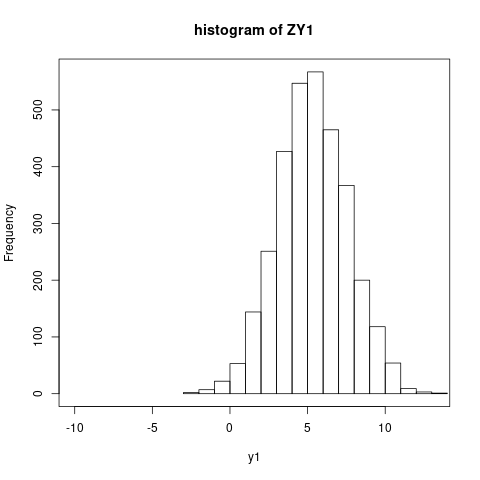
\includegraphics[width=0.3\linewidth]{../plots/two_gaussians/yone}
	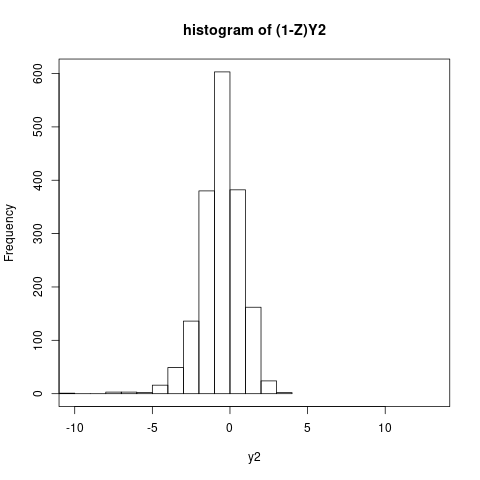
\includegraphics[width=0.3\linewidth]{../plots/two_gaussians/ytwo}
	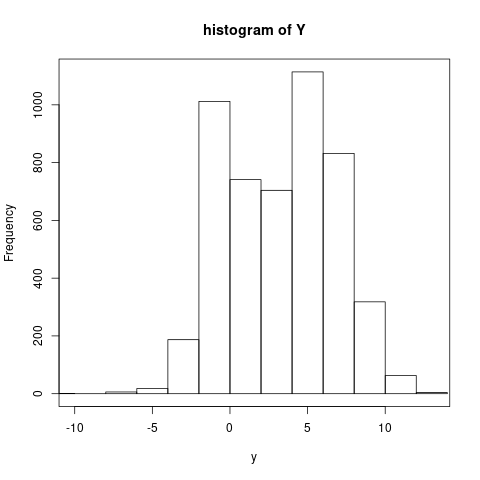
\includegraphics[width=0.3\linewidth]{../plots/two_gaussians/y}
	\caption{Distribution of $ZY,(1-Z)Y,Y$.}\label{norm-hist-y}
\end{figure}
\end{frame}

\begin{frame}{Models fitted}
Mixture of distributions (homo):
$$f(y;p,\mu,\sigma)=p_1f_N(y;\mu_1,\sigma_1^2)+(1-p_1)f_N(y;\mu_2,\sigma_2^2)$$

Mixture of linear regressions or mixture of boosting with \blue{constant} mixing probabilities (glm\_cp or boosting\_cp)
$$f(y;p,\mu,\sigma)=p_1f_N(y;\mu_1(\bx),\sigma_1^2)+(1-p_1)f_N(y;\mu_2(\bx),\sigma_2^2)$$

Mixture of linear regressions or mixture of boosting with \blue{varying} mixing probabilities (glm\_vp or boosting\_vp)
$$f(y;p,\mu,\sigma)=p_1(\bx)f_N(y;\mu_1(\bx),\sigma_1^2)+(1-p_1(\bx))f_N(y;\mu_2(\bx),\sigma_2^2)$$
\end{frame}
\begin{frame}{Results and comparisons}
	$$e_{\mu 1}=\frac{\sum_{i=1}^{n}(\mu_{i,1}-\hat{\mu}_{i,1})^2}{n}$$
	$$e_{\mu 2}=\frac{\sum_{i=1}^{n}(\mu_{i,2}-\hat{\mu}_{i,2})^2}{n}$$
	$$e_{\eta}=\frac{\sum_{i=1}^{n}(\eta_{i}-\hat{\eta}_{i})^2}{n}, \eta_i=\log\frac{p_i}{1-p_i}$$
\begin{table}[htp!]
	\centering
	\caption{Summary of test losses for different models.}\label{gaussian-summary}
	\begin{tabular}{c|rrrr}
		\hline
		model        & \multicolumn{1}{c}{neg LL} & \multicolumn{1}{c}{$e_{\mu 1}$} & \multicolumn{1}{c}{$e_{\mu 2}$} & \multicolumn{1}{c}{$e_{\eta}$} \\ \hline
		homo         & 2.5868                   & 6.2657                         & 2.6688                        & 3.3304                             \\
		glm\_cp      & 1.8978                   & 0.7775                         & 0.3233                         & 3.2440                             \\
		glm\_vp      & 1.7698                   & 0.8028                         & 0.3260                         & 1.2667                             \\
		boosting\_cp & 1.7492                   & 0.2461                         & {\bf 0.1062}                        & 3.2242                             \\
		boosting\_vp & {\bf 1.6407}                  & {\bf 0.2334}                         & 0.1105                         & {\bf 0.8435}                             \\ \hline
	\end{tabular}
\end{table}
\end{frame}
\subsection{A real data example: claims severity modelling}
\begin{frame}{Distribution of average claim amount}
Claims amount data {\tt freMTPL2sev} from R package {\bf CASdatasets}. Sample size $n=24,938$. \blue{Three peaks and heavy tail}.
\begin{figure}[h!]
	\centering
	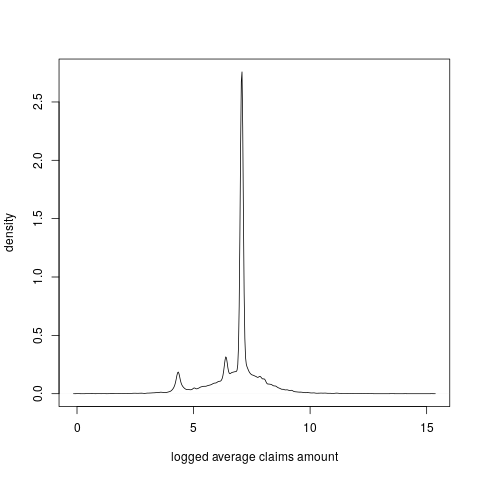
\includegraphics[width=0.35\linewidth]{../plots/sev/hist.png}
	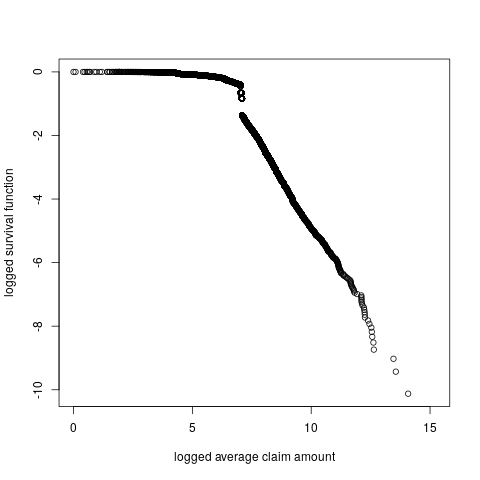
\includegraphics[width=0.35\linewidth]{../plots/sev/log-log.png}
	\caption{Histogram and logged survival function of logged average claims.}\label{tail}
\end{figure}
\end{frame}

\begin{frame}{Mixture of distributions}
Three gamma distributions for three peaks. One gamma distribution for resting non-tail part. One Pareto distribution for tail.
$$f(y)=\sum_{k=1}^4p_kf_{gamma}(y;\mu_k,\phi_k)+p_5f_{pareto}(y;\alpha,M)$$
where $\mu,\phi$ are mean and dispersion parameter, and $\alpha, M$ are tail index and threshold. The threshold is pre-determined as $8158.13$ according to Hill plot.
\end{frame}

\begin{frame}{Initialization of hidden variable}

Figure \ref{tail} indicates a way to initialize the hidden variable:
\begin{equation}
	\begin{aligned}
		\hat{z}^{[0]}_i&=(\hat{z}^{[0]}_{i,1},\hat{z}^{[0]}_{i,2},\hat{z}^{[0]}_{i,3},\hat{z}^{[0]}_{i,4},\hat{z}^{[0]}_{i,5})^\top\\
		&=(\mathbbm{1}_{(0,500]}y_i,\mathbbm{1}_{(500, 1000]}y_i,\mathbbm{1}_{(1000,1200]}y_i,\mathbbm{1}_{(1200,8158.13]}y_i,\mathbbm{1}_{(8158.13,\infty)}y_i)^\top
	\end{aligned}
\end{equation}

Other parameters can be initialized as the MLE based on the full likelihood function.

\end{frame}


\begin{frame}{EM algorithm}
	\begin{figure}[h!]
		\centering
		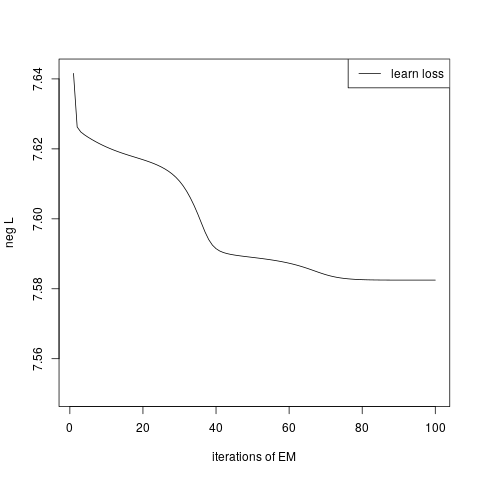
\includegraphics[width=0.35\linewidth]{../plots/sev/null_trace}
		\caption{Learning loss of mixture of distributions.}\label{null_sev}
	\end{figure}
\end{frame}

\begin{frame}{Estimated parameters}	\begin{table}[h!]
		\centering
		\caption{MLE of four component gamma distributions. Tail index is estimated as $\hat{\alpha}=1.0773$}\label{null-gamma}
		\begin{tabular}{crrrr}
			\hline
			component $k$ & \multicolumn{1}{c}{$\mu_k$} & \multicolumn{1}{c}{shape $(1/\phi_k)$} & \multicolumn{1}{c}{scale} & \multicolumn{1}{c}{rate} \\ \hline
			1         & 76.8727                & 105.556                   & 0.7283                    & 1.3731                   \\
			2         & 592.5909               & 653.539                   & 0.9067                    & 1.1029                   \\
			3         & 1171.3811              & 999.9999                  & 1.1714                    & 0.8537                   \\
			4         & 1534.5143              & 1.0377                    & 1478.7768                 & 7e-04                    \\ \hline
		\end{tabular}
	\end{table}

~

Those large shape parameters (small dispersion) implies the difficulties with \blue{gamma mean modeling}.
\end{frame}

\begin{frame}{Boosting mixing probabilities}
	$$f(y|\bx)=\sum_{k=1}^4p_k(\bx)f_{gamma}(y;\mu_k,\phi_k)+p_5(\bx)f_{pareto}(y;\alpha,M)$$
\begin{figure}[htp!]
	\centering
	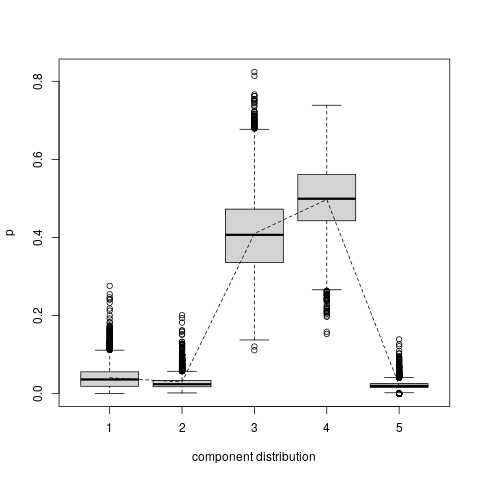
\includegraphics[width=0.35\linewidth]{../plots/sev/glm_p}
	\caption{Boxplot of estimated mixing probabilities.}\label{glm-p}
\end{figure}
\end{frame}

\begin{frame}{Boosting the forth component  mean}
$$
\begin{aligned}
f(y|\bx)=&\sum_{k=1}^3p_k(\bx)f_{gamma}(y;\mu_k,\phi_k)+ \\
&p_4(\bx)f_{gamma}(y;\mu_4(\bx),\phi_4)+ p_5(\bx)f_{pareto}(y;\alpha,M)
\end{aligned}
$$
Test loss (negative log-likelihood)
\begin{enumerate}
	\item Mixture of distributions:
	7.5815
	\item Boosting mixing probabilities:
	{\bf 7.5588}
	\item Boosting mixing probabilities and the forth component mean:
	7.5573.
\end{enumerate}
\end{frame}

\section{Conclusions}
\begin{frame}{Our proposal: Expectation-Boosting algorithm}
	Expectation-Boosting (EB) algorithm:
	\begin{itemize}
		\item Replaces the maximization step by an \blue{overfitting-sensitive} boosting step.
		\item The boosting step follows a \blue{generic functional gradient descent algorithm}.

	\end{itemize}
\end{frame}

\begin{frame}{Advantages}
	Several advantages of EB algorithm over the EM algorithm.
	\begin{itemize}
		\item No need for specifying the form of component regression functions and performing covariate transformation.
		\item Only need for component \blue{loss functions}.
		\item Boosting algorithm is a flexible non-parametric regression facilitating both \blue{non-linear effects and interaction}.
		\item  Boosting algorithm is \blue{overfitting-sensitive}, we can perform \blue{variable selection} simultaneously during the EB algorithm.
	\end{itemize}
\end{frame}

\section*{}
\begin{frame}
	\centering
	\Huge{Thank you! \\Q \& A}
\end{frame}

\end{document}
